In this section, we summarize the work related to the subject of this thesis. Apart from the papers discussing searching for optimal connections and earliest arrivals in time-dependent scenarios, we also briefly summarize the research done on route planning in road networks and on distance oracles in general. \\

\subsection{Distance oracles and route-planning}

	\noindent We have already mentioned in section~\ref{sec:prel} the paper of \textbf{Thorup and Zwick}~\cite{apxdo05} where the term ``distance oracle'' originated. The authors have shown that given an undirected weighted graph of $n$ vertices and $m$ edges and a chosen integer $k \geq 1$, we can build a distance oracle such that:
	\begin{itemize}
    	\item preprocessing takes $O(kmn^{1/k})$ expected time
        \item resulting distance oracle is of size $O(kn^{1 + 1/k})$
        \item answering queries takes $O(k)$ time
        \item stretch is at most $2k - 1$ 
	\end{itemize}
	\hspace{\fill}
	
	\noindent Moreover, the authors have reasoned that their construction is essentially optimal with respect to space - i.e., if we want to have exact and constant-time answers, we will in general be forced to pre-compute $\Omega(n^2)$ information. The parameter $k$ however provides a nice option to make trade-offs between the four parameters, as depicted on figure~\ref{fig:compr}.\\
	
	\begin{figure}[h!]
        \begin{center}
			\inputTikZ{./tikzpics/compromises}
        \end{center}
		\caption{\label{fig:compr} By moving $k$ (decreasing on the picture), we can achieve compromises between the four parameters of the distance oracle.}
	\end{figure}
	
	\noindent Another work by \textbf{Gavoille} et al.~\cite{distlabel04} concerned distance labelling - a somewhat restricted version of a distance oracle where we assign each node in the graph its distance label. This is again only some pre-computed information and upon a query from $x$ to $y$, we should be able to figure out their distance only using the corresponding distance labels. In the paper it is shown that for all $n$, there exist infinitely many graphs of $n$ vertices for which we have an exact distance labelling scheme of a small overall size ($\mathcal{O}(n \log n)$), but for which the process of figuring out the distance from the labels takes too long from practical point of view. \\
	
	\noindent Even though these results imply that we cannot create a sufficiently small efficient distance oracle in general, it may still be possible for sub-classes of general graphs, or even better, for a single particular graph. In that respect, the road network is the point of interest and fortunately it has a few ``nice'' properties (it is sparse, almost planar, the maximum node degree is small...) which made it possible to design exact and efficient algorithms with extremely fast query times. To name a few of these:
	\begin{itemize}
		\item \textbf{Highway hierarchies} (2005, \cite{hwhierarchies05}). The preprocessing of the algorithm works in iterations - in each of them the edges of little importance are pruned, the remaining graph is contracted (long chains of edges are replaced with shortcuts) and the result forms the new layer, connected to the previous one, and used as an input for the next iteration. On such hierarchy of layers, bidirectional Dikstra's algorithm is run, climbing up the hierarchy in each direction.
		\begin{itemize}
			\item Speed-up: about 2500
			\item Techniques: hierarchy, shortcuts, bidirectional Dijkstra
		\end{itemize}
		\item \textbf{Transit node routing} (2006, \cite{transit06}). The algorithm completely replaces searching with table look-ups. There is a small set of transit nodes between which the exact distance is stored in a table. Also each node remembers its nearest transit nodes (called access nodes~\footnote{This served partly as an inspiration for our algorithm \textit{USP-OR-A} discussed in section~\ref{sec:usp}.}) and the their distance. A search is necessary only in case of a local query. A disadvantage is a bigger space consumption.
		\begin{itemize}
			\item Speed-up: more than 1 000 000
			\item Techniques: landmarks
		\end{itemize}

		\begin{figure}[h!]
		\centering
		\makebox[0pt][c]{
	    \begin{minipage}{0.45\textwidth}  
		    \centering
		    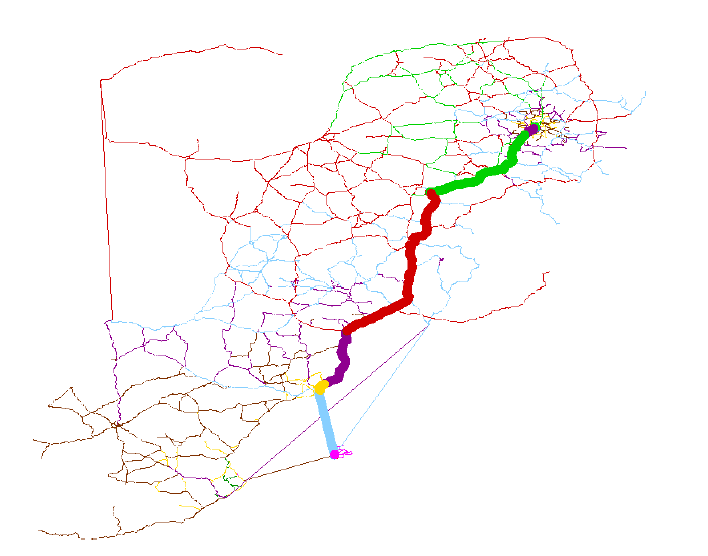
\includegraphics[width=5cm]{hwhier.png}
	    \end{minipage}
		\hspace{1cm}
	    \begin{minipage}{0.45\textwidth} 
	    	\centering
		    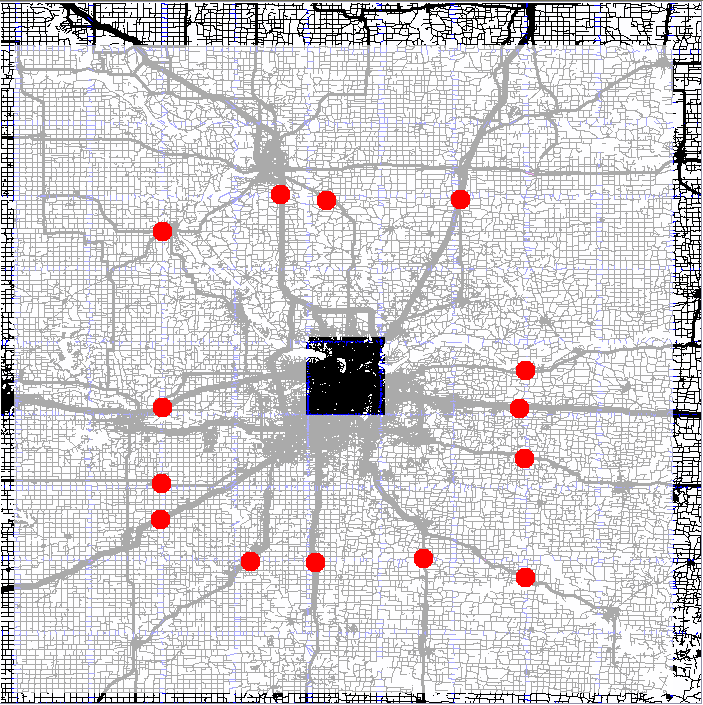
\includegraphics[width=5cm]{transitnodes.png}
	    \end{minipage}
	    }
	    \caption{\label{fig:hwhier} Highway hierarchies (left) - the bidirectional Dijkstra search climbs up the hierarchy to reach the most sparse level. Transit node routing (right) - access nodes (in red) that cannot be avoided when going ``out of town''.}
		\end{figure}
		
		\item \textbf{Contraction hierarchies} (2008, \cite{contracthier08}). The preprocessing creates additional shortcut edges in the graph. This is done by deleting one by one the vertices of the original graph and adding shortcuts where necessary - to preserve original distances. The quality depends mostly on the order in which we delete the vertices. Upon a query, a bidirectional Dijkstra search is run on the original graph enriched with the added shortcuts. The algorithm is less memory demanding than Transit node routing.
		\begin{itemize}
			\item Speed-up: more than 30 000
			\item Techniques: shortcuts (contractions), bidirectional Dijkstra
		\end{itemize}
	\end{itemize}
	\hspace{\fill}
	
	\begin{figure}[h!]
		\centering
		\makebox[0pt][c]{
	    \begin{minipage}{0.45\textwidth}  
		    \centering
		    \inputTikZ{./tikzpics/contraction}
	    \end{minipage}
		\hspace{1cm}
	    \begin{minipage}{0.45\textwidth} 
	    	\centering
		    \inputTikZ{./tikzpics/contractionaft}
	    \end{minipage}
	    }
	    \caption{\label{fig:contraction} Deleting vertex $E$ in Contraction hierarchies. Before (left) and after (right).}
		\end{figure}
	
	\noindent One thing these methods have in common is that their query time is very low in practice, but it is not guaranteed theoretically. This was the point of interest in the work~\cite{highwaydim10}, which introduces a parameter called \textit{highway dimension}. The authors show that a low highway dimension guarantees good query times of many route-planning algorithms, including the three we have mentioned. \\
	
	\noindent A very good summary of the techniques devised for road network route-planning up to the year 2009 can be found in~\cite{engineeringroute09}. Efficient distance oracles are also known for graphs with small recursive separators~\cite{distlabel04}. The work~\cite{sommerthesis10} suggests efficient distance oracle for power-law graphs and another distance oracle method for general graphs, offering trade-offs between stretch and query times. It also gives an exhaustive and comprehensive discussion regarding shortest path queries in general, which we point out to interested readers.
	
\subsection{Time-dependent scenario}
	
	The time-dependent scenario has so far seen much smaller speed-ups than static routing in road networks, one reason for this being that the adaptation of the many techniques used for road networks to the time-dependent scenario is not so straightforward. This is mainly due to the fact that running bidirectional Dijkstra's algorithm (commonly used with static route-planning techniques) in time-dependent networks requires the knowledge of the destination time~\cite{engtimeexp09}. All the same, for some methods this adaptation was carried out with good results:
	\begin{itemize}
		\item \textbf{Time-dependent contraction hierarchies} (2009,~\cite{timedepch09}). The focus in this case was on road networks having time-dependent edge weights (e.g. due to morning congestions) and on computing earliest arrival value for a given query. The main difference between the static Contraction hierarchies is that the backward search is run from more arrival times of the destination node. Each such run may then contribute a new lower or upper bound for the actual earliest arrival value, based on if the forward and backward search met (a solution was found).
		\begin{itemize}
			\item Speed-up (TD road-network, 18 million nodes): up to 2000
		\end{itemize}
		\item \textbf{Time-dependent SHARC} (2008,~\cite{sharc08}). Static SHARC is an algorithm using unidirectional Dijkstra, it was therefore a good candidate to be adjusted for time-dependent scenario. It combines several techniques, perhaps the most important being pre-computing arc flags (\cite{arcflags06}) for a multi-partitioned graph, which is basically information stating if the given arc should/should not be considered when travelling to the destination cell.
		\begin{itemize}
			\item Speed-up (TD road-network, 5 million nodes): up to 800
			\item Speed-up (timetable, 30 000 stations): up to 27
		\end{itemize}
		\item \textbf{Engineering TE graphs...} (2009,~\cite{engtimeexp09}). While the previous papers used the time-dependent model of the timetable, this work concentrates on the time-expanded model. On a high level, this model is further refined by bypassing some low degree nodes, remodelling unimportant stations and introducing time-dependent shortcuts - still in the phase of preprocessing. During the query, additional speed-up techniques are deployed to reduce the search space explored by Dijkstra's algorithm, as this can get quite huge in time-expanded graphs.
		\begin{itemize}
			\item Speed-up (timetable, 30 000 stations): up to 57
		\end{itemize}
	\end{itemize}
	\hspace{\fill}
	
	\noindent A summary of some time-dependent route planning techniques (up to year 2009) can be found in~\cite{tdroute09}. The paper~\cite{timetablemodelsalgs07} discusses also multi-criteria queries and gives an overview of comparisons between time-dependent and time-expanded timetable model. 